\chapter*{Introduction Générale}
\label{chap:intro}
\addcontentsline{toc}{chapter}{\nameref{chap:intro}}

\section{Contexte et Motivations}
\label{sec:intro:contexte}
Une décision jurisprudentielle peut être définie soit comme  le résultat rendu par des juges à l'issue d'un procès, ou bien un document décrivant une affaire judiciaire. Un tel document rapporte, en fait,  les faits, les procédures judiciaires, la solution des juges, et les raisons qui les y ont conduits. Dans ce mémoire, nous désignons par \og décision \fg{} le document, et par  \og résultat\fg{} la conclusion, ou réponse, ou solution finale des juges. Une jurisprudence\footnote{\url{http://www.toupie.org/Dictionnaire/Jurisprudence.htm}} est un ensemble de décisions rendues par les tribunaux et qui représente la manière dont ces derniers interprètent les lois pour résoudre un problème juridique donné (type de contentieux). Les juristes doivent collecter ces documents, en sélectionner et analyser pour leurs études. En effet, leur analyse aide à mieux comprendre la prise de décision des juridictions, par exemple, pour des recherches empiriques en droit \citep{ancel2003expulsion, jeandidier2006pensions}. Les avocats exploitent aussi les décisions passées pour anticiper les résultats des juges. Ils peuvent ainsi mieux conseiller leurs clients sur le risque judiciaire que ces derniers encourent, et sur la stratégie à adopter dans un contentieux. Cette activité de collecte et d'analyse est manuelle en général, et par conséquent, sujette à plusieurs difficultés liées à l'accès aux données et à l'exhaustivité de cette analyse. 

Les documents sont dispersés entre les tribunaux. Les procédures administratives ne facilitent pas toujours leur accès du fait de la nécessité de préserver la confidentialité des parties. Les décisions n'étant pas anonymisées ne peuvent être rendues aux juristes qui en font la demande. Un certain nombre de documents sont néanmoins accessibles sur internet grâce à des sites de publication de données ouvertes gouvernementales comme \url{data.gouv.fr} qui applique progressivement la loi sur les données ouvertes ??? en publiant régulièrement les décisions récentes.  Il existe aussi des moteurs de recherche juridique qui permettent d'effectuer de retrouver des décisions intéressantes. Cependant, qu'ils soient payant (LexisNexis, dalloz, lamy,...) ou gratuits (legifrance), leurs critères de recherche limitent la pertinence des résultats. En effet, il ne s'agit en général que de combinaisons de mots-clés et autres métadonnées (date, type de juridiction, ...), ou d'expressions régulières, comme l'illustre la Figure \ref{fig:intro:juriSearchForm}. Ces critères manquent la sémantique juridique qui ramènerait, aux juristes, des échantillons plus pertinents. 

\begin{figure}
	\centering
	\begin{subfigure}[t]{0.95\textwidth}
		\centering
		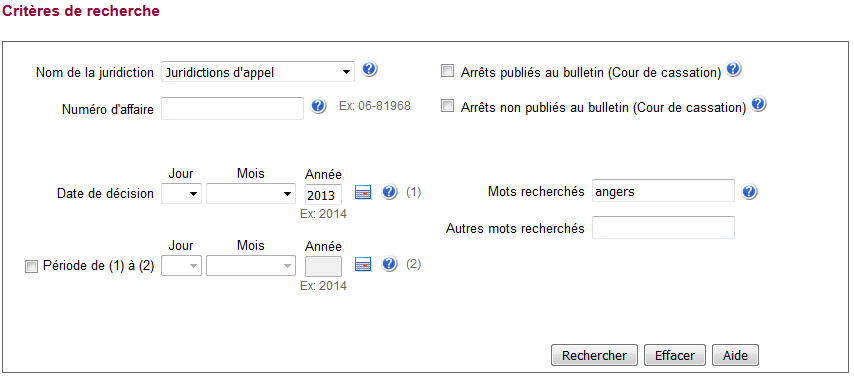
\includegraphics[width=0.9\textwidth]{legifrance.PNG}
		\caption{\url{www.legifrance.gouv.fr}}
	\end{subfigure}%

	\begin{subfigure}[t]{0.45\textwidth}
		\centering
		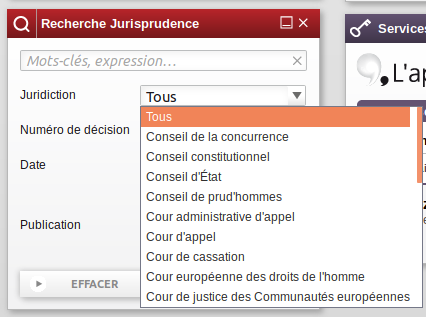
\includegraphics[scale=0.4]{dalloz.png}
		\caption{\url{www.dalloz.fr}}
	\end{subfigure}\hfill
	\begin{subfigure}[t]{0.55\textwidth}
		\centering
		\fbox{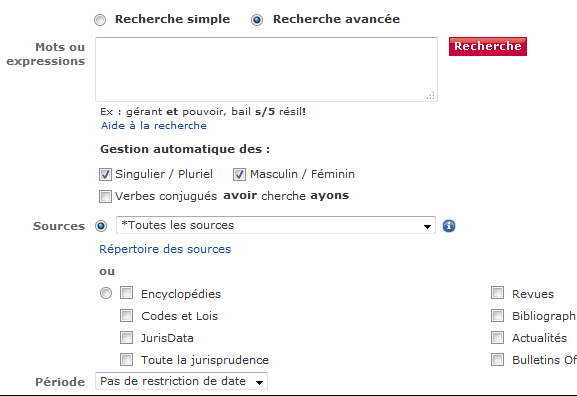
\includegraphics[scale=0.35]{lexisnexis.png}}
		\caption{\url{www.lexisnexis.com}}
	\end{subfigure}%
	\caption{Exemples de critères des moteurs de recherche juridique}\label{fig:intro:juriSearchForm}
\end{figure}

L'exhaustivité de l'analyse, ou tout au moins sa représentativité, rencontre un frein face à l'énorme volume existant de documents. En effet, plus de 4 millions de décisions sont prononcées en France par an d'après les chiffres du ministère français de la justice (Tableau \ref{tab:intro:nbdecisionstats}). Au regard de la croissance rapide de la quantité de décisions, on imagine facilement que même pour une étude sur une question très précise, le corpus utile reste large. Par ailleurs, il peut s'avérer très pénible de lire les décisions pour en identifier les données d'intérêt. Les documents sont très souvent longs. Ils sont aussi complexes dans leur style de rédaction. Par exemple, les phrases sont longues et comprennent plusieurs clauses discutant parfois d'aspects différents. On y retrouve aussi des références à des jugements antérieurs, et des omissions, ...
\begin{table}
\small
\begin{center}
\begin{tabular}{|l|l|l|l|l|l|}
	\hline
\textbf{Justice}	& \textbf{2013}      & \textbf{2014}      & \textbf{2015}      & \textbf{2016}      & \textbf{2017}      \\ \hline
	civile         & 2 761 554 & 2 618 374 & 2 674 878 & 2 630 085 & 2 609 394 \\ \hline
	pénale         & 1 303 469 & 1 203 339 & 1 206 477 & 1 200 575 & 1 180 949 \\ \hline
	administrative & 221 882   & 230 477   & 228 876   & 231 909   & 242 882   \\ \hline
\end{tabular}

\textit{\scriptsize{Source: \url{http://www.justice.gouv.fr/statistiques-10054/chiffres-cles-de-la-justice-10303/}}}  
\end{center}
\caption{Nombre de décisions prononcées en France par an de 2013 à 2017}\label{tab:intro:nbdecisionstats}
\end{table}


%\textcolor{red}{Introduire l'utilité de l'automatisation}
Il est évident qu'une automatisation du traitement des corpus de décisions s'impose pour répondre aux diverses difficultés d'accès, de volumétrie, et de complexité liées à la compréhension des décisions. L'idée est de faire gagner du temps aux juristes sur des tâches d'aide à leur raisonnement d'experts, tout en leur fournissant une vue pertinente de la jurisprudence autant sur le plan sémantique que synthétique. Par ailleurs, \citet{cretin2014justicecomplexe} fait remarquer que la justice est complexe dans son organisation (Figure \ref{orgjusticefrance}) et son fonctionnement, et son langage est presque incompréhensible. Il est donc difficile aux profanes d'estimer leurs droits et le risque judiciaire qu'ils encourent dans leur quotidien sans consulter un initié en droit. L'automatisation pourrait aussi améliorer l'accessibilité du droit dans ce cas.  L'exigence pour le profane étant l'exacte pertinence des ressources, leur accessibilité, et l'intuitivité du processus de leur exploitation \citep{narazenko2017legalnlpintro}. Le traitement automatique constitue en résumé une aide précieuse non seulement pour les professionnels du droit, mais aussi pour les particuliers et entreprises soucieux de les chances que l'issue d'un procès, les impliquant, leur soit favorable. Une telle information a une valeur inestimable car elle les aiderait par exemple à se décider entre un arrangement à l'amiable et la poursuite de leur offenseur en justice \citep{langlaischappe2009ecoresolutionlitige}.

\begin{figure}
	\centering 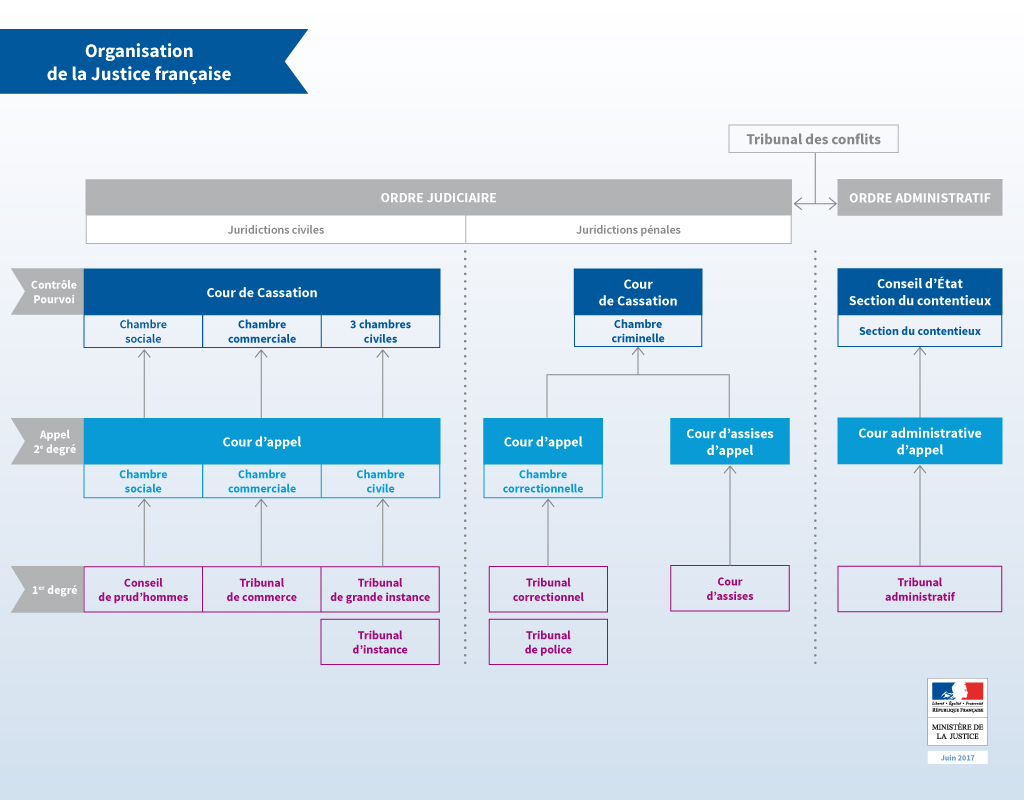
\includegraphics[width=0.9\textwidth]{organisation_justice_francaise_grand.jpg}
	
	\textit{\scriptsize{Source: \url{http://www.justice.gouv.fr/organisation-de-la-justice-10031/}}}  
	\caption{Organisation des institutions judiciaires françaises} \label{orgjusticefrance}
\end{figure}

\section{Objectifs}
%\textcolor{red}{Description d'une approche traditionnelle, exemple d'études, difficultés de ces études}
 Ce mémoire discute des résultats d'une étude visant à automatiser l'extraction d'information à partir des décisions afin de faciliter la recherche, et les analyses descriptives et prédictives d'un corpus jurisprudentiel. L'approche traditionnelle d'analyse d'un contentieux ou d'une demande \citep{ancel2003expulsion} consiste à :
 \begin{enumerate}
 	\item \textbf{choisir un échantillon représentatif}: collection des décisions suivant des contraintes définies:  période précise et d'une couverture géographique, types d'affaires (types d' évidents et types marginaux), diversité, hétérogénéité. 
 	\item \textbf{Sélectionner les décisions}: élimination des décisions qui ne correspondent pas au type de demande d'intérêt.
 	\item \textbf{Elaborer la grille d'analyse}: création d'un modèle de grille (tableau) qui permettra d'enregistrer les informations "potentiellement importantes". Chaque ligne correspond à une demande et les colonnes sont les différents types d'informations qu'on peut extraire sur une demande. Ces variables vont de la procédure suivie, aux solutions proposées en passant par la nature de l'affaire. Les champs à remplir ne sont pas connus à l'avance; c'est la lecture des décisions qu'on retrouve les informations qui paraissent intéressant à observer.
 	\item \textbf{L'analyse des décisions et l'interprétation des informations}: saisie des décisions et statistique sur un logiciel tableur comme MS Excel pour généralement observer la répartition des décisions suivant.
 \end{enumerate}
 
\citet{ancel2003expulsion} évoque principalement le problème de la différence entre l'état capté de la jurisprudence et son état présent. En effet, Les longs délais de travail sont caractéristiques de ces études. Nous avons pour exemple, l'analyse empirique des déterminants de la fixation de pensions alimentaires pour enfant lors de divorce réalisée par l'équipe de Bruno Jeandidier \citep{jeandidier2006pensions}. Cette analyse a duré 9 mois pour l'extraction manuelle des informations et la modélisation par régression de la relation entre les déterminant extraits et les pensions alimentaires accordées.  D'autre part, il est impossible d'observer l'évolution des pratiques judiciaires dans le temps et dans l'espace du fait de la faible taille de l'échantillon choisie. Notre principal objectif est donc de proposer des solutions pour un traitement rapide et efficace d'une grande masse de décisions. 
 
 La question à la base de notre étude est celle de savoir \og comment capter automatiquement la sémantique d'un corpus jurisprudentiel pour comprendre la prise de décision des juges sachant que l'interprétation subjective des règles juridiques rend l'application de la loi non déterministe ? \fg{}. Cette question intéresse des entreprises telles que LexisNexis, et plusieurs startups  à l'exemple de Predictice\footnote{\url{http://predictice.com}} et CASE LAW ANALYTICS\footnote{\url{http://caselawanalytics.com}}. Afin d'y répondre, nous nous intéressons  aux concepts manipulés par les experts au centre desquels on retrouve la demande ou prétention des parties. Tout autour de la demande, gravitent d'autres concepts importants qui enrichissent la compréhension de la décision (Figure \ref{fig:intro:demande-central}): 
 \begin{itemize}
	\item le résultat associé qui est décrite par une polarité (\og accepte \fg{} ou \og rejette \fg{}), souvent un quantum accordé (par ex. 5000 euros, 2 mois d'emprisonnement);
	\item le fondement ou la norme juridique qui est la règle qui détermine et légitime la prétention ou le résultat;	
	\item l'objet qui représente ce qui a été demandé (par ex. dommages et intérêts);
	\item les circonstances factuelles 	dans lesquelles sont formulées les demandes; ils décrivent les types de faits caractérisant ainsi les types de contentieux ou d'affaires;
	\item les raisons c'est-à-dire les divers arguments apportés par les parties (resp. les juges) pour justifier leurs requêtes (resp. leurs solutions);
 \end{itemize}

\begin{figure}
    \centering
    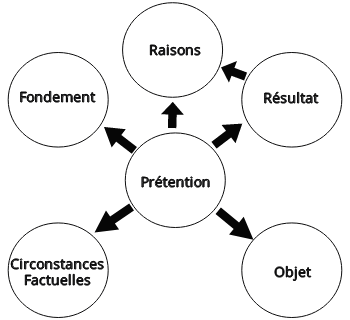
\includegraphics[scale=0.85]{demande-central.png}
    \caption{La demande au centre de la compréhension des décisions}
    \label{fig:intro:demande-central}
\end{figure}

En fait, cette abstraction couvre l'essentiel de l'information pertinente pour les experts.  L'analyse sémantique vise donc à identifier les connaissances sur les nombreuses demandes présentent dans les décisions. 

Les travaux de cette thèse s'inscrivent dans un projet qui vise, entre autres, l'automatisation de l'analyse empirique des contentieux pour observer de manière exhaustive et synthétique les pratiques judiciaires. L'objectif final est d'obtenir un système capable de fournir une estimation des chances d'obtenir un résultat positif suivant des critères comme la juridiction, le type de demande, ainsi que les faits du contentieux, et d'identifier les facteurs influençant le résultat. Le projet comprend deux phases principales : une phase d'indexation des connaissances de la masse des décisions, suivie d'une phase d'analyse prédictive. La phase d'indexation doit déjà permettre de réaliser automatiquement, de manière plus exhaustives, des analyses descriptives.Ces dernières consistent par exemple à comparer le nombre d'acceptations à la fréquence des rejets, comparer les quanta demandés et accordés, analyser l'évolution temporelle et la différence spatiale de la prise de décision dans les juridictions. Par conséquent, le système doit apprendre à reconnaître dans les décisions, les informations pertinentes sur les prétention et résultats associés. Pour la phase d'analyse prédictive, le principe consiste à regrouper des paquets de décisions homogènes (même résultat sur la même prétention dans les circonstances similaires), pour découvrir les facteurs influençant le sens du résultat (par ex. le fait que \og le revenu de l'époux soit le plus élevé du foyer\fg{} encourage les juges à accorder la pension alimentaire à l'épouse). En effet, c'est la connaissance de ces facteurs qui permet à l'expert de pouvoir anticiper les décisions judiciaires. La chaîne de traitement à mettre en \oe uvre consiste en quatre étapes principales qui s'enchaînent comme le présente la figure \ref{fig:intro:pipeline-globale}. 
\begin{figure}
	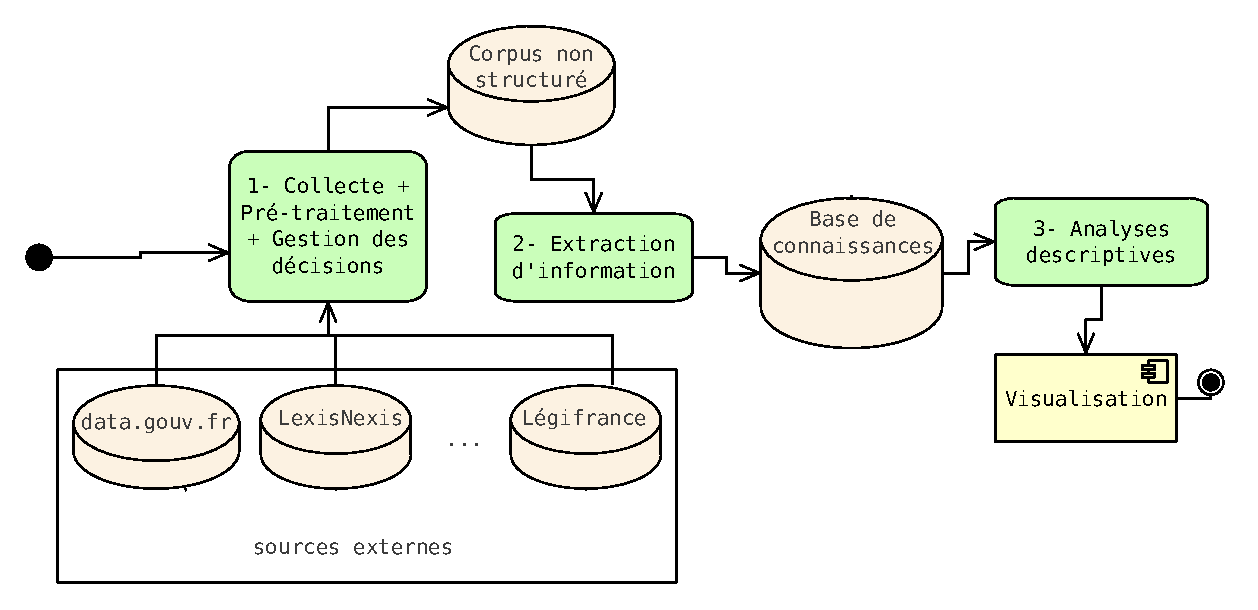
\includegraphics[width=\textwidth]{pipeline-cassandra.pdf}
	\caption{Chaine d'analyse du corpus jurisprudentiel à mettre en \oe uvre} \label{fig:intro:pipeline-globale}
\end{figure} 

Ce mémoire n'aborde pas l'aspect prédictif du projet. Notre étude s'est limitée aux problématiques liées à l'analyse descriptive, et qui sont décrites dans la section suivante.

\section{Problématiques d'analyse descriptive}
\label{sec:intro:probleme}

Les analyses descriptives exigent de répondre à diverses problématiques techniques dont les principales sont décrites dans les sous-sections suivantes.

\subsection{Collecte, gestion et pré-traitement des documents}

Malgré le fait que les décisions de justice civile sont les premières visées, ce projet a l'ambition de couvrir la majorité des juridictions des 1er et 2nd degrés. Le volume de décisions prononcées est énorme et croit très rapidement (table \ref{tab:intro:nbdecisionstats}). Il est donc nécessaire de trouver des moyens pour collecter le maximum de documents bruts non-structurés, les pré-traiter, et aussi organiser leur gestion afin de les indexer en local pour faciliter leur traitement.

Les décisions de cours d'appel de la justice civile sont les plus accessibles à partir des moteurs de recherche juridique (LexisNexis, 
Dalloz, LamyLine, Legifrance, ...) et de la grande base de données JURICA de la Cour de cassation. Cependant, l'accès à ces décisions est généralement payant et Le nombre de documents simultanément téléchargeables est très faibles sur les sites payants (généralement 10 à 20 décisions au maximum à la fois). En plus, le nombre de téléchargements par jour est limité. La base JURICA forunit la plus grosse base de décisions de cours d'appel (justice civile) en France. Elle est gérée par la Cour de cassation. L'accès à cette base est offert par Le service de documentation, des études et du rapport\footnote{\url{https://www.courdecassation.fr/institution_1/composition_56/etudes_rapport_28.html}} (SDER). Cet accès est payant pour les professionnels et gratuit pour les universités et centres de recherche en partenariat avec le SDER. L'accès public et gratuit est fourni principalement par Legifrance, le moteur de recherche juridique du ministère de la justice. Les décisions y sont identifiées à l'aide de numéros consécutifs et accessibles à partir d'un service web à l'aide d'une requête GET du protocole HTTP. Ainsi, à l'aide d'une boucle, il est possible de programmer un client web capable de télécharger l'ensemble des documents de Legifrance. LegiFrance a cet avantage de proposer des décisions de tous les ordres et de tous les degrés. Cependant, les décisions des juridictions du premier (jugements) restent plus rares sur internet et pincipalement disponibles auprès des tribunaux et autres juridictions de premier jugement.  La facilité d'accès au décisions du second degré ou d'appel (arrêts) en justice civile est l'une des raisons pour lesquelles notre étude s'est portée sur ceux-ci.

Les décisions existent sous divers formats PDF, DOC, DOCX, RTF, TXT, XML,... Il arrive parfois qu'un fichier téléchargé comprenne plusieurs décisions (sur LexisNexis par ex.). Nous avons par conséquent préférer convertir tous les documents au simple format plein texte pour homogénéiser pls facilement les traitement. Par ailleurs, les décisions sont collectées à partir de diverses sources pouvant contenir des documents identiques. Le stockage pose donc le problème d'identification unique des décisions pour éviter des redondances. Pour cela, nous avons défini un schéma de nomination unique des fichiers. Ce dernier repose sur 3 informations: le type de juridiction (tribunal, cour d'appel, ...), la ville, et le numéro R.G. (registre général: l'identifiant unique de la décision au sein de la juridiction). Par exemple, le numéro \og CAREN1606137 \fg{} identifie la décision de numéro R.G. \og 16/06137 \fg{} de la cour d'appel (\og CA \fg{}) de la ville de Rennes (\og REN \fg{}). D'autre part, certains moteurs de recherche ne fournissent souvent qu'un résumé au lieu du contenu original des décisions. Il est important de  supprimer les fichiers de résumé du corpus.

\subsection{Extraction d'information}

\subsection{Standardisation et représentation des données}
La phase de représentation des connaissances porte sur la structuration effective des décisions dans la base de connaissance. Il est nécessaire de définir préalablement un schéma des données/connaissances qui permettra d'expliciter les éléments et les relations à enregistrer, et le type de requête qu'on peut effectuer sur la base. Ce schéma définit en fait les types de concepts et de liens dont les instances sont les informations extraites des textes.

D'autre part, la base doit avoir une représentation qui permette de la connectée à des bases externes pour élargir les analyses possibles (par ex. l'observation de la distribution de décisions par région/département nécessite de savoir à quelle région/département appartient chaque ville de la base, mais cette information est absente des textes).

\subsection{Recherche d'information}
Comment retrouver des décisions similaires à une situation donnée exprimée à l'aide d'un formulaire ou d'une description en langage naturel? La structuration du corpus permet de sélectionner les critères ou propriétés du type d'affaires qu'on veut analyser. Pour permettre une plus grande expressivité de la situation, on pourrait envisager le cas où un particulier, par exemple, voudrait décrire son problème de manière naturelle à l'aide de phrases\footnote{Exemple de situation décrite en langage naturel: \url{http://www.documentissime.fr/questions-droit/question-46724-emprunt-et-divorce.html}}. L'objectif serait dans un premier temps de retrouver les décisions de la base de connaissances qui paraissent similaires à la situation décrite. Ensuite, l'utilisateur  peut s'aider des modèles prédictifs pour effectuer des analyses.

L'automatisation réussi-t-elle à combler les limites de l'approche traditionnelle (par ex. observation de l'évolution des pratiques judiciaires dans le temps).

On s'attend à ce que les catégories de situations (d'affaires) soient suggérées de manière non supervisée par regroupement automatique (hiérarchique si possible). Après avoir filtrer les demandes suivant les catégories prédéfinies de demandes, il faudrait suggérer des catégories de faits pour regrouper de manières non supervisée les décisions (demandes) des demandes sélectionnées. Avec une structuration fine, on pourrait voir si avec seulement les faits on y arrive ou si on on a besoin de tout le texte.


\section{Méthodologie}
\label{sec:intro:methodologie}
%Proposition d'approches taillées sur mesure et conçues par combinaison et adaptation des techniques établies de la la bibliographie.


Les problématiques propres aux textes juridiques trouvent généralement des analogies avec les problématiques de recherche en analyse de données textuelles. Ainsi l'énorme progrès réalisé dans ce domaine a permis d'obtenir de nombreuses approches transposable au textes juridiques. Cependant, l'adaptation est généralement nécessaire pour obtenir des résultats de bonne qualité hors des domaines pour lesquels ces approches ont été développées \citep{Waltl2016lexia}. De plus, la recherche en analyse de données se fait sur des données qui n'illustrent généralement pas la réelle complexité des données réelles. Etant donné que nous avons effectué l'une des premières études d'analyse de jugements français, nous avons axé notre travail sur le rapprochement des problématiques techniques liées à l'analyse des décisions jurisprudentielles aux problématiques généralement traitées en analyse de données textuelles en général. Il s'agissait ensuite d'établir des protocole d'évaluation et d'annotations nécessaires de données nécessaires. Selon les problématiques identifiées et les protocoles d'évaluations définies, des techniques établies de la littérature ont été adaptés et expérimentés sur les données réelles annotées par des experts.

\section{Résultats}
\label{sec:intro:résultats}
Le projet vise à fournir des outils d'extraction d'information afin de contribuer à la création de nouvelles vues, perspectives et représentations des décisions de justices. Ces outils doivent plus distinctement permettre d'analyser de manière descriptive et prédictive, résumer dans une structure sémantique propre au domaine judiciaire, explorer, visualiser en terme de différence spatiale et d'évolution temporelle, l'énorme corpus de décisions jurisprudentielles qui croit rapidement d'année en année.

\section{Structure du mémoire}
\label{sec:intro:organisation}

\textbf{Chapitre \ref{chap:literature}} \\[0.2em]
%blindtext

\textbf{Chapitre \ref{chap:structuration}} \\[0.2em]
%\blindtext

\textbf{Chapitre \ref{chap:quanta}} \\[0.2em]
%\blindtext

\textbf{Chapitre \ref{chap:sensresultat}} \\[0.2em]
%\blindtext

\textbf{Chapitre \ref{chap:similarite}} \\[0.2em]
%\blindtext

\textbf{Chapitre \ref{chap:conclusion}} \\[0.2em]

\textbf{Les annexes \ref{chap:demo}} \\[0.2em]
